\documentclass[11pt]{article}
\usepackage[utf8]{inputenc}
\usepackage[T1]{fontenc}     % Fix weird character
\usepackage{geometry}
\usepackage{amsmath}
\usepackage{amssymb}
\usepackage{gensymb}
\usepackage{spalign}
\usepackage{xfrac}
\usepackage{parskip}
\usepackage{float}  % figure[H]
\usepackage[style=ieee,backend=biber]{biblatex}
\usepackage[breaklinks=true,bookmarks=true,hidelinks]{hyperref}
\usepackage{tikz}
\usepackage{pgfplots}
\pgfplotsset{compat=newest,compat/show suggested version=false}

\geometry{
    a4paper,
    hmargin=2.54cm,
    tmargin=1.27cm,
    bmargin=1.27cm,
    includeheadfoot
}
\setcounter{secnumdepth}{0}  % Disable section numbering

\begin{filecontents}{fourier_series.bib}
@misc{wiki:sq_wave,
    author = "{Wikipedia contributors}",
    title = "Square wave --- {Wikipedia}{,} The Free Encyclopedia",
    year = "2023",
    url = "https://en.wikipedia.org/w/index.php?title=Square_wave&oldid=1170692196",
    note = "[Online; accessed 14-November-2023]"
}
@misc{wiki:tr_wave,
    author = "{Wikipedia contributors}",
    title = "Triangle wave --- {Wikipedia}{,} The Free Encyclopedia",
    year = "2023",
    url = "https://en.wikipedia.org/w/index.php?title=Triangle_wave&oldid=1173717071",
    note = "[Online; accessed 14-November-2023]"
}
@misc{wiki:sa_wave,
    author = "{Wikipedia contributors}",
    title = "Sawtooth wave --- {Wikipedia}{,} The Free Encyclopedia",
    year = "2023",
    url = "https://en.wikipedia.org/w/index.php?title=Sawtooth_wave&oldid=1139895676",
    note = "[Online; accessed 14-November-2023]"
}
\end{filecontents}
\addbibresource{fourier_series.bib}

\newcommand{\SquareWaveBuilder}[2]{
    \edef\result{}
    \foreach \k in {1,...,#1} {
        \ifnum\k=1
            \xdef\result{sin((2*\k-1)*#2)/(2*\k-1)}
        \else
            \xdef\result{\result+sin((2*\k-1)*#2)/(2*\k-1)}
        \fi
    }
    4*(\result)/pi
}
\newcommand{\TriangleWaveBuilder}[2]{
    \edef\result{}
    \foreach \k in {1,...,#1} {
        \ifnum\k=1
            \xdef\result{((-1)\string^\k*sin((2*\k-1)*#2))/(2*\k-1)\string^2}
        \else
            \xdef\result{\result+((-1)\string^\k*sin((2*\k-1)*#2))/(2*\k-1)\string^2}
        \fi
    }
    -8*(\result)/pi\string^2
}
\newcommand{\SawtoothWaveBuilder}[2]{
    \edef\result{}
    \foreach \k in {1,...,#1} {
        \ifnum\k=1
            \xdef\result{((-1)\string^\k*sin(\k*#2))/\k}
        \else
            \xdef\result{\result + ((-1)\string^\k*sin(\k*#2))/\k}
        \fi
    }
    -2*(\result)/pi
}

\begin{document}
\section{Fourier series}

\subsection{Sine wave}

\begin{equation}
    x(t) = A\sin(2\pi ft + \varphi)
    \label{eq:si_wave}
\end{equation}

where $f$ is the cycle frequency over time $t$, $A$ is the amplitude and $\varphi$ is the phase.

\begin{figure}[H]
    \centering
    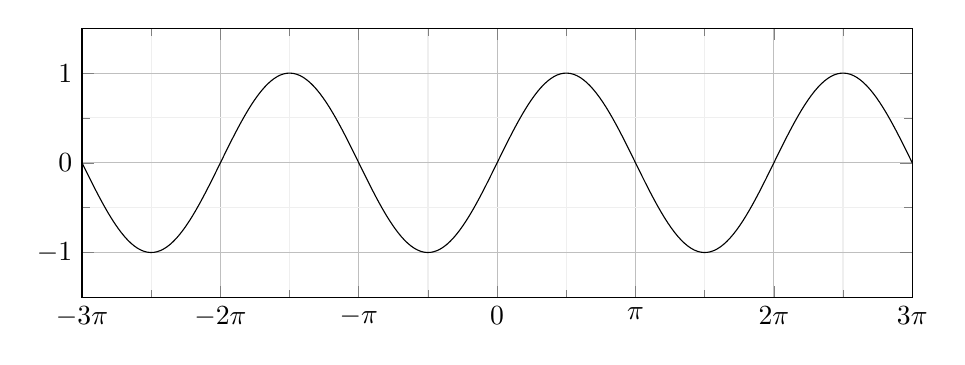
\begin{tikzpicture}
        \begin{axis}[
            xmin = -3*pi,
            xmax = 3*pi,
            ymin = -1.5,
            ymax = 1.5,
            grid = both,
            xtick distance = pi,
            minor tick num = 1,
            minor grid style = {lightgray!25},
            xticklabels = {, $-3\pi$, $-2\pi$, $-\pi$, 0, $\pi$, $2\pi$, $3\pi$},
            width  = \textwidth,
            height = 5cm
        ]
            \addplot[domain=-3*pi:3*pi,samples=256]{sin(deg(x))};
        \end{axis}
    \end{tikzpicture}
    \caption{Visualization of a sine wave with a frequency of 1 Hz and an amplitude of 1 unit, plotted in the interval $-3\pi < x < 3\pi$.}
    \label{fig:si_wave}
\end{figure}

\subsection{Square wave}

\begin{equation}
    x(t) = \frac{4}{\pi}\sum_{k = 1}^{\infty}\frac{1}{2k - 1}\sin(2\pi(2k - 1)ft)
    \label{eq:sq_wave}
\end{equation}

where $f$ is the cycle frequency over time $t$.\cite{wiki:sq_wave}

\begin{figure}[H]
    \centering
    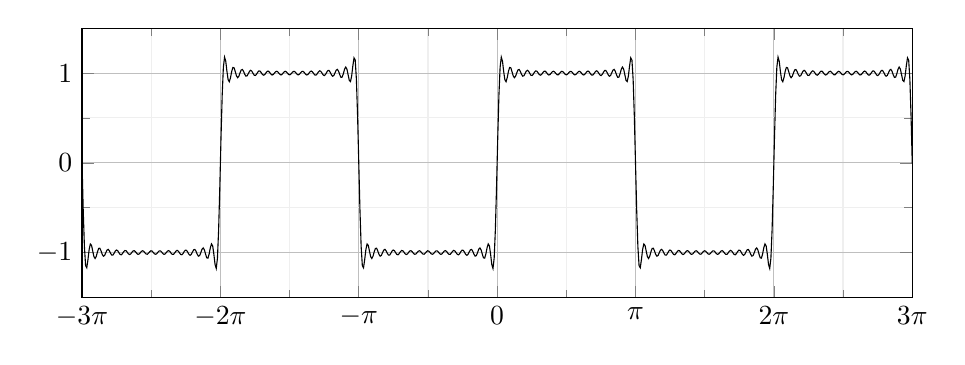
\begin{tikzpicture}
        \begin{axis}[
            xmin = -3*pi,
            xmax = 3*pi,
            ymin = -1.5,
            ymax = 1.5,
            grid = both,
            xtick distance = pi,
            minor tick num = 1,
            minor grid style = {lightgray!25},
            xticklabels = {, $-3\pi$, $-2\pi$, $-\pi$, 0, $\pi$, $2\pi$, $3\pi$},
            width  = \textwidth,
            height = 5cm
        ]
            \addplot[domain=-3*pi:3*pi,samples=700] {4*(sin((2*1-1)*deg(x))/(2*1-1)+sin((2*2-1)*deg(x))/(2*2-1)+sin((2*3-1)*deg(x))/(2*3-1)+sin((2*4-1)*deg(x))/(2*4-1)+sin((2*5-1)*deg(x))/(2*5-1)+sin((2*6-1)*deg(x))/(2*6-1)+sin((2*7-1)*deg(x))/(2*7-1)+sin((2*8-1)*deg(x))/(2*8-1)+sin((2*9-1)*deg(x))/(2*9-1)+sin((2*10-1)*deg(x))/(2*10-1)+sin((2*11-1)*deg(x))/(2*11-1)+sin((2*12-1)*deg(x))/(2*12-1)+sin((2*13-1)*deg(x))/(2*13-1)+sin((2*14-1)*deg(x))/(2*14-1)+sin((2*15-1)*deg(x))/(2*15-1)+sin((2*16-1)*deg(x))/(2*16-1))/pi};
        \end{axis}
    \end{tikzpicture}
    \caption{Visualization of a square wave function with max iteration of 16, with $f = 1\ \mathrm{Hz}$ and amplitude of 1.}
    \label{fig:sq_wave}
\end{figure}

% \SquareWaveBuilder{16}{deg(x)}

\newpage
\subsection{Triangle wave}

\begin{equation}
    x(t) = -\frac{8}{\pi^2}\sum_{k=1}^{\infty}\frac{(-1)^k}{(2k - 1)^2}\sin(2\pi(2k - 1)t)
    \label{eq:tr_wave}
\end{equation}

where $f$ is the cycle frequency over time $t$.\cite{wiki:tr_wave}

\begin{figure}[H]
    \centering
    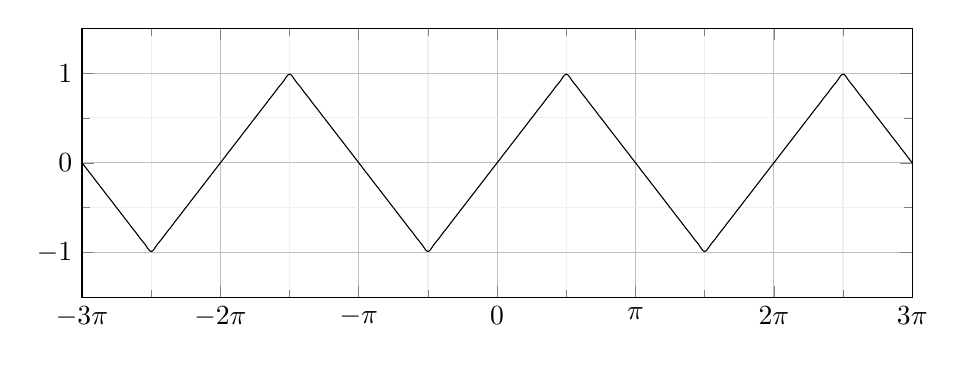
\begin{tikzpicture}
        \begin{axis}[
            xmin = -3*pi,
            xmax = 3*pi,
            ymin = -1.5,
            ymax = 1.5,
            grid = both,
            xtick distance = pi,
            minor tick num = 1,
            minor grid style = {lightgray!25},
            xticklabels = {, $-3\pi$, $-2\pi$, $-\pi$, 0, $\pi$, $2\pi$, $3\pi$},
            width  = \textwidth,
            height = 5cm
        ]
            \addplot[domain=-3*pi:3*pi,samples=700] {-8*(((-1)^1*sin((2*1-1)*deg(x)))/(2*1-1)^2+((-1)^2*sin((2*2-1)*deg(x)))/(2*2-1)^2+((-1)^3*sin((2*3-1)*deg(x)))/(2*3-1)^2+((-1)^4*sin((2*4-1)*deg(x)))/(2*4-1)^2+((-1)^5*sin((2*5-1)*deg(x)))/(2*5-1)^2+((-1)^6*sin((2*6-1)*deg(x)))/(2*6-1)^2+((-1)^7*sin((2*7-1)*deg(x)))/(2*7-1)^2+((-1)^8*sin((2*8-1)*deg(x)))/(2*8-1)^2+((-1)^9*sin((2*9-1)*deg(x)))/(2*9-1)^2+((-1)^10*sin((2*10-1)*deg(x)))/(2*10-1)^2+((-1)^11*sin((2*11-1)*deg(x)))/(2*11-1)^2+((-1)^12*sin((2*12-1)*deg(x)))/(2*12-1)^2+((-1)^13*sin((2*13-1)*deg(x)))/(2*13-1)^2+((-1)^14*sin((2*14-1)*deg(x)))/(2*14-1)^2+((-1)^15*sin((2*15-1)*deg(x)))/(2*15-1)^2+((-1)^16*sin((2*16-1)*deg(x)))/(2*16-1)^2)/pi^2};
        \end{axis}
    \end{tikzpicture}
    \caption{Visualization of a triangle wave function with max iteration of 16, with $f = 1\ \mathrm{Hz}$ and amplitude of 1.}
    \label{fig:tr_wave}
\end{figure}

% \TriangleWaveBuilder{16}{deg(x)}

\subsection{Sawtooth wave}

\begin{equation}
    x(t) = -\frac{2}{\pi}\sum_{k = 1}^{\infty}\frac{(-1)^k}{k}\sin(2\pi kft)
    \label{eq:sa_wave}
\end{equation}

where $f$ is the cycle frequency over time $t$.\cite{wiki:sa_wave}

\begin{figure}[H]
    \centering
    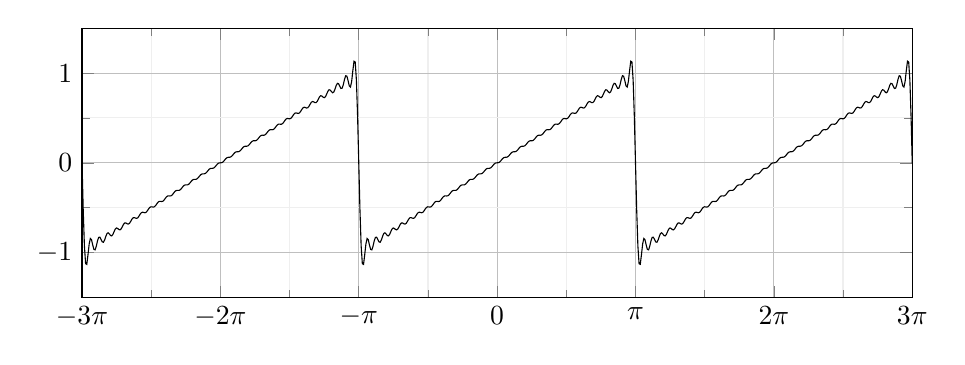
\begin{tikzpicture}
        \begin{axis}[
            xmin = -3*pi,
            xmax = 3*pi,
            ymin = -1.5,
            ymax = 1.5,
            grid = both,
            xtick distance = pi,
            minor tick num = 1,
            minor grid style = {lightgray!25},
            xticklabels = {, $-3\pi$, $-2\pi$, $-\pi$, 0, $\pi$, $2\pi$, $3\pi$},
            width  = \textwidth,
            height = 5cm
        ]
            \addplot[domain=-3*pi:3*pi,samples=700] {-2*(((-1)^1*sin(1*deg(x)))/1+ ((-1)^2*sin(2*deg(x)))/2+ ((-1)^3*sin(3*deg(x)))/3+ ((-1)^4*sin(4*deg(x)))/4+
((-1)^5*sin(5*deg(x)))/5+ ((-1)^6*sin(6*deg(x)))/6+ ((-1)^7*sin(7*deg(x)))/7+ ((-1)^8*sin(8*deg(x)))/8+
((-1)^9*sin(9*deg(x)))/9+ ((-1)^10*sin(10*deg(x)))/10+ ((-1)^11*sin(11*deg(x)))/11+ ((-1)^12*sin(12*deg(x)))/12+
((-1)^13*sin(13*deg(x)))/13+ ((-1)^14*sin(14*deg(x)))/14+ ((-1)^15*sin(15*deg(x)))/15+ ((-
1)^16*sin(16*deg(x)))/16+ ((-1)^17*sin(17*deg(x)))/17+ ((-1)^18*sin(18*deg(x)))/18+ ((-1)^19*sin(19*deg(x)))/19+
((-1)^20*sin(20*deg(x)))/20+ ((-1)^21*sin(21*deg(x)))/21+ ((-1)^22*sin(22*deg(x)))/22+ ((-
1)^23*sin(23*deg(x)))/23+ ((-1)^24*sin(24*deg(x)))/24+ ((-1)^25*sin(25*deg(x)))/25+ ((-1)^26*sin(26*deg(x)))/26+
((-1)^27*sin(27*deg(x)))/27+ ((-1)^28*sin(28*deg(x)))/28+ ((-1)^29*sin(29*deg(x)))/29+ ((-
1)^30*sin(30*deg(x)))/30+ ((-1)^31*sin(31*deg(x)))/31+ ((-1)^32*sin(32*deg(x)))/32)/pi};
        \end{axis}
    \end{tikzpicture}
    \caption{Visualization of a sawtooth wave function with max iteration of 32, with $f = 1\ \mathrm{Hz}$ and amplitude of 1.}
    \label{fig:sa_wave}
\end{figure}

% \SawtoothWaveBuilder{32}{deg(x)}

\newpage
\printbibliography
\end{document}

